\documentclass{article}
\usepackage{setspace,tikz,wrapfig}
\usepackage[text={6.5in,8.5in},centering]{geometry}
\geometry{verbose,a4paper,tmargin=2.4cm,bmargin=2.4cm,lmargin=2.4cm,rmargin=2.4cm}
\usepackage{graphicx,amsmath,cases,multirow,appendix,graphicx,xcolor}
\usepackage[makeroom]{cancel}

\setlength\parindent{0pt}

\newcommand{\note}[1]{\colorbox{gray!30}{#1}}
\newcommand{\ind}{\-\hspace{1cm}}
\newcommand*\circled[1]{\tikz[baseline=(char.base)]{
            \node[shape=circle,draw,inner sep=2pt] (char) {#1};}}
\newenvironment{rcases}
  {\left.\begin{aligned}}
  {\end{aligned}\right\rbrace} 
  
  
\renewcommand\floatpagefraction{.9}
\renewcommand\topfraction{.9}
\renewcommand\bottomfraction{.9}           


\begin{document}

\noindent\makebox[\textwidth][c]{\Large\bfseries Lecture 16 -- Press perturbations}

\textbf{Concepts:}\\
\ind - Formalize pulse vs. press perturbations\\
\ind - Community matrix vs. Interaction matrix\\
\ind - Net Effects matrix (direct, indirect, vs. net effects)

\rule[0.5ex]{\linewidth}{1pt}
So far dealing explicitly with pulse perturbations:\\
\ind Q was: How will system respond?

\ind \emph{Pulse} - `instantaneous', one-time acute change in population size (or factor affecting growth rates)\\
\ind\ind Watched how system, including perturbed spp., responded.
\begin{center}
 	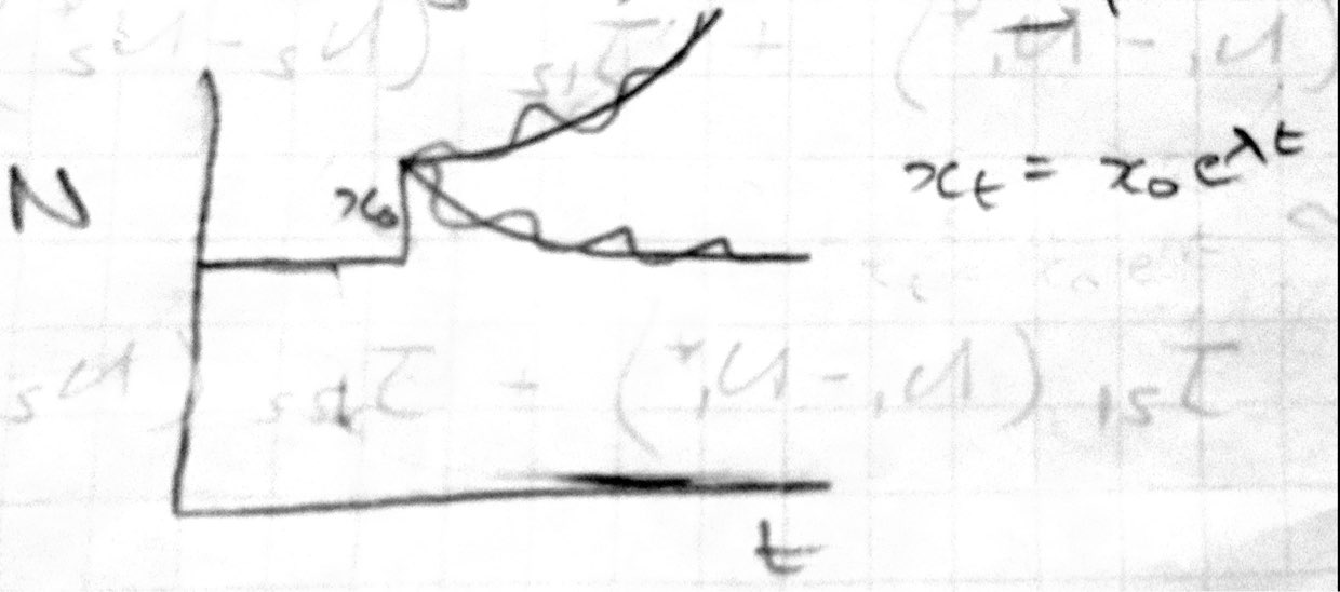
\includegraphics[width=3cm]{figs/Pulse.pdf}
\end{center}
\ind \ind $\Rightarrow$ Empirically relevant for invasibility or pulse-like disturbances\\
\ind \ind \ind (Note importance of spp. generation time)\\

\textbf{Today:}  \emph{Press} perturbations\\
\ind (Often-misused term by empiricists)\\
\ind \ind Chronic, sustained change in growth rate or abundance\\
\ind \ind \ind e.g., continuous addition/removal of individuals at a constant rate\\
\ind \ind \ind e.g., change in parameters contributing to $\frac{dN}{dt}$\\
\ind \ind \ind e.g., change in abundance of focal species (held to new abundance)\\
\ind \ind No complete species removals!\\

\ind Will assume: \\
\ind \ind (1) Fixed point equilibrium coexistence before and after\\
\ind \ind (2) No species goes extinct\\
\ind \ind (3) No bifurcations crossed (e.g., no Hopf bifurcation to limit cycles)\\
\ind  \ind $\Rightarrow$ Sufficiently small perturbations between nearby fixed point equilibria

\rule[0.5ex]{\linewidth}{1pt}
\textbf{Review Jacobian and Taylor expansion}\\
For 1-sp.:
\begin{equation*}
	\frac{dN}{dt}=F(N)=N\cdot f(N) \qquad \qquad f \text{ can be highly nonlinear}
\end{equation*}
\ind Approximate $F(N)$ with 1st-order Taylor expansion around $N^*$.
\begin{align*}
	F(N^*+x_0)=F(N^*+(N-N^*))=F(N^*) + \frac{F'(N^*)}{1!}(N-N^*)+ h.o.t.
\end{align*}
\ind Since by definition $F(N^*)=0$ \& ignoring $h.o.t.$...
\begin{align*}
 \approx F'(N^*)(N-N^*) = F'(N^*)x_0 = \left.\frac{d\tfrac{dN}{dt}}{dN}\right\vert_{N^*} \cdot x_0 = \lambda x_0
\end{align*}

For 2-spp.:
\begin{align*}
	\frac{dN_1}{dt}=F_1(N_1,N_2) \qquad \frac{dN_2}{dt}=F_2(N_1,N_2)
\end{align*}
\ind Taylor expansion around $(N_1^*, N_2^*)$...
\begin{align*}
	F_1(N_1+x,N_2+y)=\cancelto{0}{F_1(N_1^*,N_2^*)} & + F_1'(N_1^*)(N_1-N_1^*) +... \\
	... & + F_1'(N_2^*)(N_2-N_2^*) + h.o.t.\\
	& \approx \underbrace{\left.\frac{\partial F_1}{\partial N_1}\right\vert_{(N_1^*,N_2^*)}}_{A_{11}}(N_1-N_1^*) + \underbrace{\left.\frac{\partial F_1}{\partial N_2}\right\vert_{(N_1^*,N_2^*)}}_{A_{12}}(N_2-N_2^*)\\
	& \approx A_{11}(N_1-N_1^*) + A_{12}(N_2-N_2^*)
\end{align*}
Similarly for 2nd species:
\begin{align*}
F_2(N_1+x,N_2+y)  \approx A_{21}(N_1-N_1^*) + A_{22}(N_2-N_2^*)
\end{align*}

Thus in general for $S$ species:
\begin{equation*}
	F_i(\vec{N} + \vec{n}) \approx \sum_{k=1}^S A_{ik}(N_k-N_k^*)
\end{equation*}

And in matrix form:
\begin{equation*}
	F(\vec{N}+\vec{n}) \approx \mathbf{A} \vec{n} \qquad \qquad \text{where } \vec{n}=\vec{N}-\vec{N^*}
\end{equation*}

Vector $\vec{n}$ = pulse perturbations - one-time additions/subtractions\\
\ind $\Rightarrow$ eigenvalues, trace, determinant $\Rightarrow$ \emph{asymptotic stability} etc.

\rule[0.5ex]{\linewidth}{1pt}

\textbf{Press perturbations}\\
Assume we're starting at fixed-point coexistence steady state $\vec{N}^*$ and add chronic perturbation to $N_1$:
\begin{equation*}
	\frac{dN_1}{dt}=F_1(\vec{N}^*)+P_1 \qquad \qquad  \frac{dN_2}{dt}=F_2(\vec{N}^*)
\end{equation*}
\ind $P_1$ = adding $P$ individuals of $N_1$ \textbf{per time}\\

Assume system will come to a new steady state, $N^{**}$\\

$\Rightarrow$ Taylor expand $F_1(\vec{N}^*)$ around $N^{**}$
\begin{align*}
	F_1(\vec{N}^{**}+(\vec{N}^*-\vec{N}^{**})) & \approx \cancelto{0}{F_1(N^{**})} +  P_1 + A_{11}(N_1^*-N_1^{**}) + A_{12}(N_2^*-N_2^{**})\\
	& = 0 \text{ assuming new system is at steady state}
\end{align*}
Therefore, rearranging and generalizing to include $S$ species:
\begin{align*}
	-P_1 &= \sum_{k=1}^S A_{ik}(N_k^*-N_k^{**})
\end{align*}
In matrix form,
\begin{align*}
	-\mathbf{I}\cdot \vec{P}&= \mathbf{A} \cdot \vec{n}^*\\
	-\begin{bmatrix} P_1 & 0\\0 & 0 \end{bmatrix}&=\begin{bmatrix} A_{11} & A_{12}\\A_{21} & A_{22} \end{bmatrix} \underbrace{\begin{bmatrix} N_1^* - N_1^{**} \\ N_2^* - N_2^{**}	\end{bmatrix}}_{\text{Our interest}}
\end{align*}
Want to know how much $i^{th}$ species $N_2$ changes given a press perturbation $P_j$ to species $j=1$?

\rule[0.5ex]{\linewidth}{1pt}
Can't divide by a matrix.  Use \textbf{Matrix inverse}!\\
\ind By def., $\mathbf{A}\cdot \mathbf{A}^{-1}=\mathbf{I}$
Example:
\begin{align*}
	\begin{bmatrix} 7 & 8 \\ 6 & 7 \end{bmatrix} \cdot \begin{bmatrix} ? & ? \\ ? & ? \end{bmatrix}& = \begin{bmatrix}1 & 0\\0 & 1 \end{bmatrix}\\
	\begin{bmatrix} 7 & 8 \\ 6 & 7 \end{bmatrix} \cdot \begin{bmatrix} w & x \\ y & z \end{bmatrix} &= \begin{bmatrix}1 & 0\\0 & 1 \end{bmatrix}
\end{align*}
Corresponds to 4 equations with 4 unknowns.  $\Rightarrow$ solvable!
\begin{align*}
	7 w + 8 y = 1\\
	7 x + 8 z = 0\\
	6 w + 7 y = 0\\
	6 x + 7 z = 1
\end{align*}
In \textbf{R}: \emph{solve}(A) or \emph{ginv}(A) from MASS package\\
In Mathematica: \emph{Inverse}[A] or use \emph{Solve}\\  \note{$\implies Mathematica$}
\begin{align*}
	\begin{bmatrix} 7 & 8 \\ 6 & 7 \end{bmatrix} \cdot \begin{bmatrix} 7 & -8 \\ -6 & 7 \end{bmatrix} =\begin{bmatrix} 49-48 & 56-56 \\ 42-42 & -48+49 \end{bmatrix}= \begin{bmatrix}1 & 0\\0 & 1 \end{bmatrix}
\end{align*}
Thus rewrite:
\begin{align*}
	\mathbf{A}\cdot \vec{n}^*&=-\mathbf{I}\cdot \vec{P}\\
	\mathbf{A}\cdot \vec{n}^*&=-\mathbf{A}^{-1}\mathbf{A}\cdot \vec{P}\\
	 \vec{n}^*&=-(\mathbf{A}^{-1})\cdot \vec{P}\\
\end{align*}
\begin{equation*}
	n_i^* = -\sum_{k=1}^S(\mathbf{A}^{-1})_{ik}\cdot P_j
\end{equation*}
Or, derived in terms of derivatives and a perturbation $p_j$ of any kind:
\begin{align*}
	\frac{\partial N_i^*}{\partial p_j}=-\sum_{k=1}^S(\mathbf{A}^{-1})_{ik}\cdot \frac{\partial F_k}{\partial p_j}
\end{align*}
Example in 3-spp. system:
\begin{align*}
	\frac{\Delta N_1^*}{P_2}=-\underbrace{\begin{bmatrix} A_{11}^{(-1)} & A_{12}^{(-1)} & A_{13}^{(-1)} \\ \cdot & \cdot & \cdot   \\ \cdot & \cdot & \cdot \end{bmatrix}}_{\mathbf{A}^{-1}} \cdot \begin{bmatrix} 0 \\ P_2 \\ 0 \end{bmatrix} = -\mathbf{A}_{12}^{(-1)} \cdot P_2
\end{align*}
Elements of $-(\mathbf{A}^{-1})$ specify the \textbf{Net effect} resulting from all direct and indirect effect pathways.\\
\ind Net effect of column $j$ on row $i$. \note{Contrast to Jacobian.}

Multiple perturbations at once:  Add columns...
\begin{align*}
	 \frac{\Delta N_1^*}{P_2 \text{ and } P_3}=  -\mathbf{A}_{12}^{(-1)} \cdot P_2 \; + \; -\mathbf{A}_{13}^{(-1)} \cdot P_3
\end{align*}

\rule[0.5ex]{\linewidth}{1pt}
\textbf{Trophic Cascade} -  Build some intuition for what's going on.\\
\emph{\textbf{Self-limitation in all species}}\\
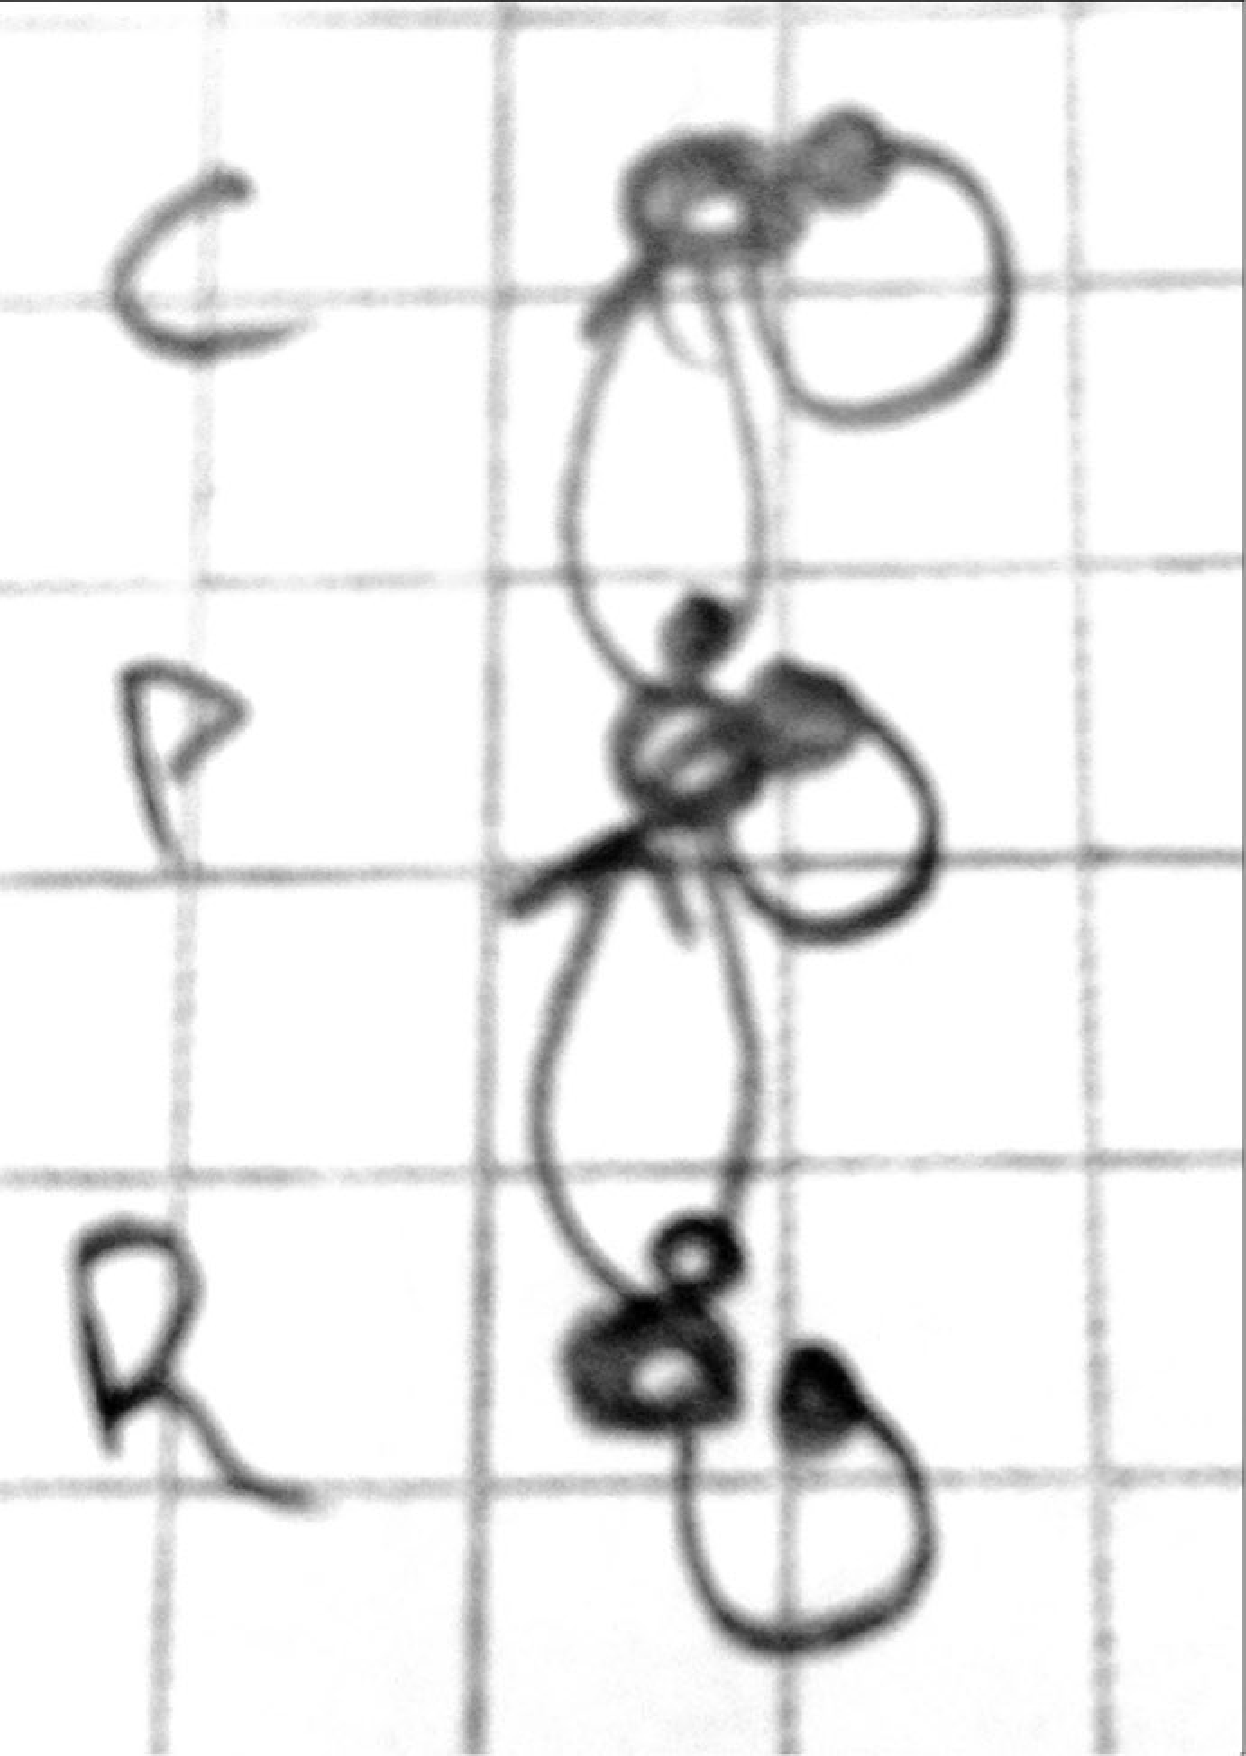
\includegraphics[width=1.25cm]{figs/TC_full.pdf}
\ind Predict perturbation to $\Rightarrow$ will cause:
\begin{align*}
\begin{matrix}
	 &	\phantom{\Rightarrow} R & \phantom{\Rightarrow}P & \phantom{\Rightarrow}C\\
	R &	\Rightarrow \uparrow & \phantom{\Rightarrow}\downarrow & \phantom{\Rightarrow} \uparrow\\
	P & \phantom{\Rightarrow}\uparrow & \Rightarrow \uparrow & \phantom{\Rightarrow}\downarrow\\
	C & \phantom{\Rightarrow} \uparrow & \phantom{\Rightarrow} \uparrow & \Rightarrow \uparrow
\end{matrix}
\end{align*}
 \note{$\Rightarrow$ Mathematica}
\begin{align*}
	\mathbf{A}=\begin{bmatrix} -1 & -1 & 0 \\ 1 & -1 & -1 \\ 0 & 1 & -1 \end{bmatrix} \qquad \Rightarrow \qquad \mathbf{-A^{-1}}=\begin{bmatrix} 2/3 & -1/3 & 1/3 \\ 1/3 & 1/3 & -1/3 \\ 1/3 & 1/3 & 2/3 \end{bmatrix} \qquad \text{matches all predictions!}
\end{align*}

But what did we observe in class last time as a function of $K$?
\begin{center}
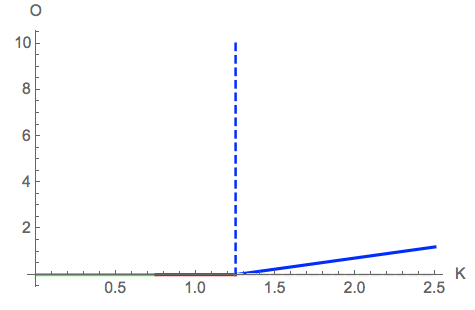
\includegraphics[width=4.5cm]{figs/TC_R.png}\ind 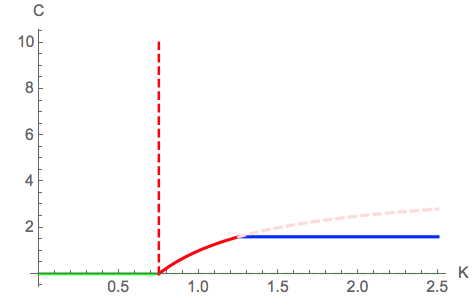
\includegraphics[width=4.5cm]{figs/TC_C.png}\ind 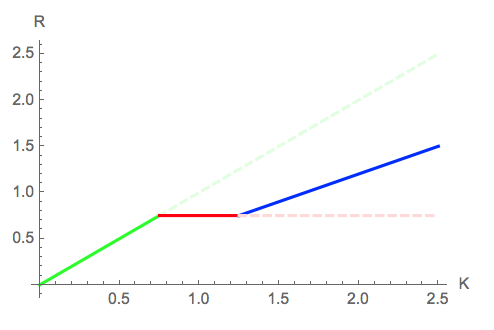
\includegraphics[width=4.5cm]{figs/TC_P.png}
\end{center}
\emph{\textbf{Self-limitation in basal species only}}\\
\ind 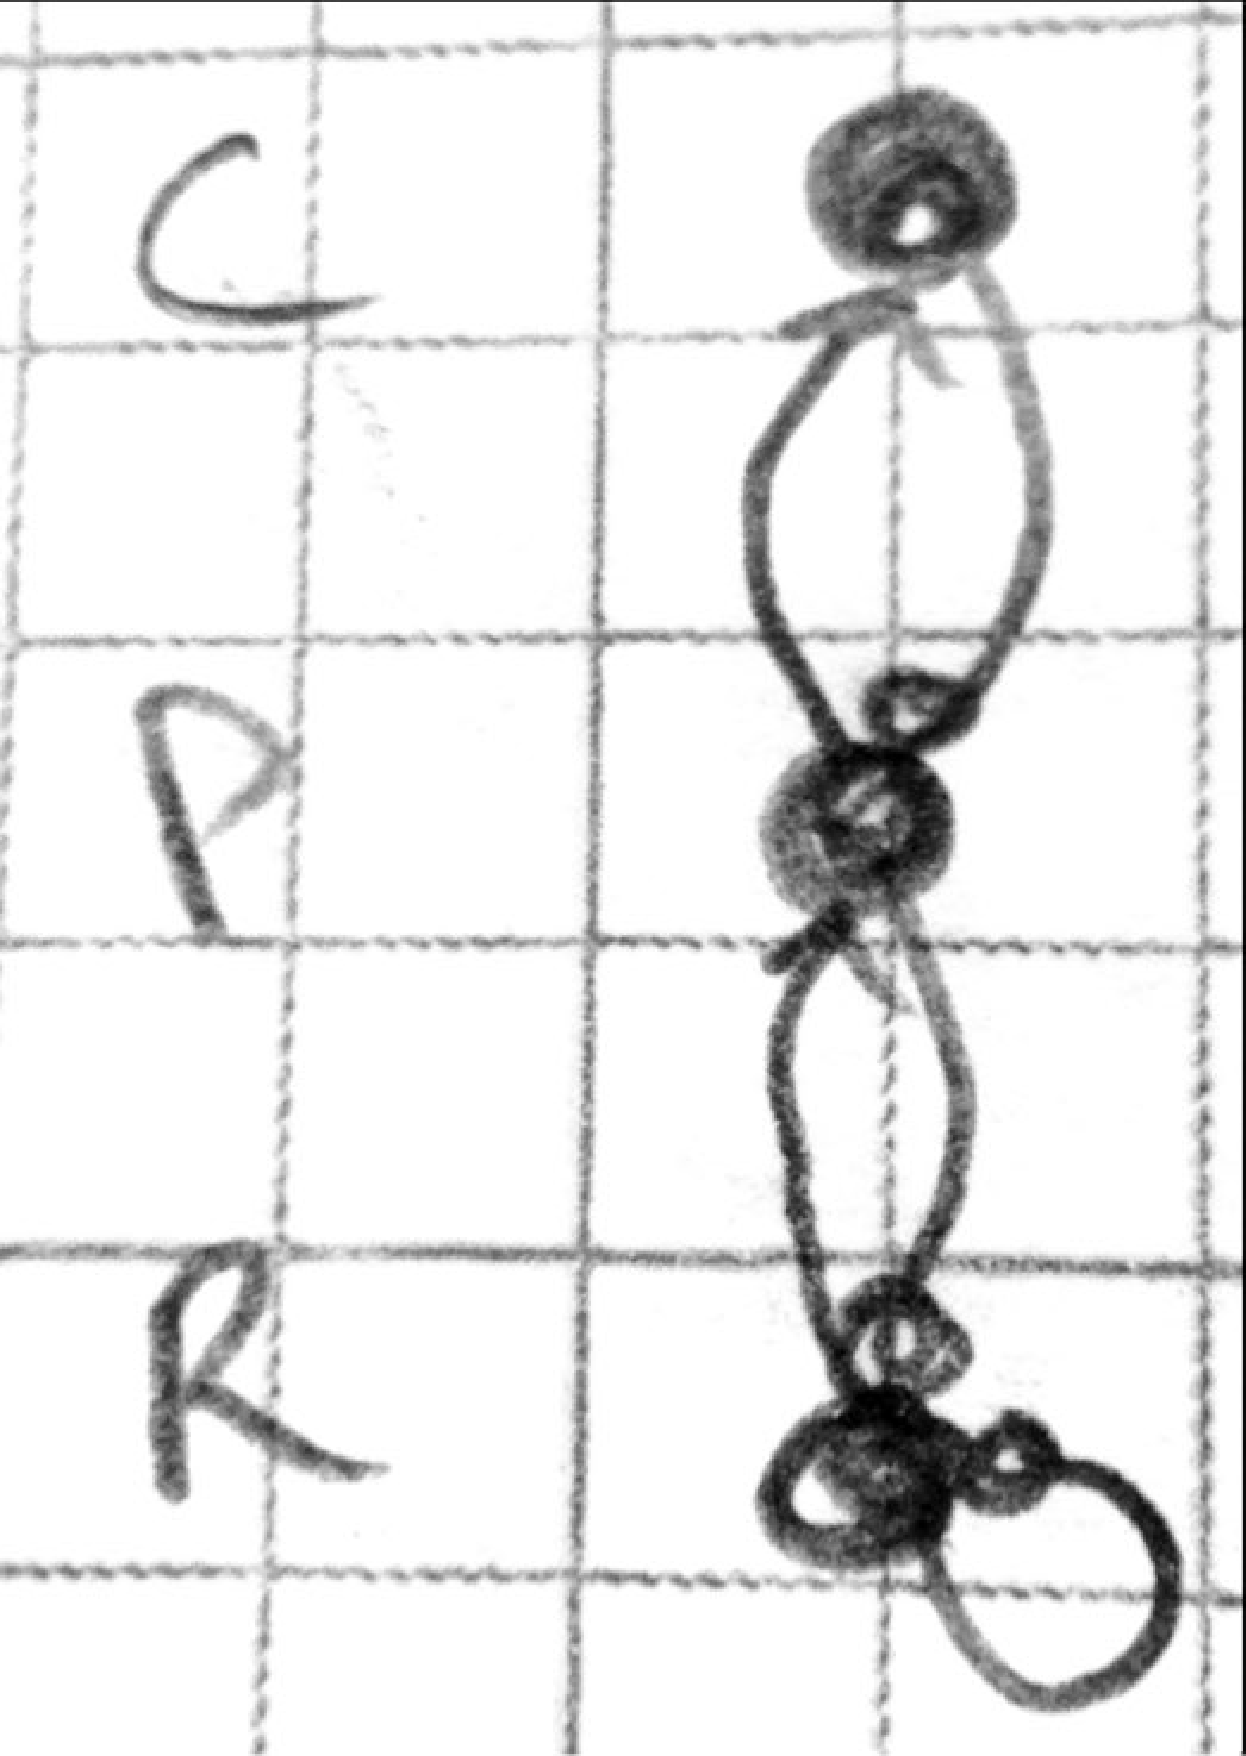
\includegraphics[width=1.25cm]{figs/TC_basal.pdf}
 \note{$\Rightarrow$ Mathematica}
\begin{align*}
	\mathbf{A}=\begin{bmatrix} -1 & -1 & 0 \\ 1 & 0 & -1 \\ 0 & 1 & 0 \end{bmatrix} \qquad \Rightarrow \qquad \mathbf{-A^{-1}}=\begin{bmatrix} 1 & 0 & 1 \\ 0 & 0 & -1 \\ 1 & 1 & 1 \end{bmatrix} \qquad \text{matches all predictions!}
\end{align*}


\rule[0.5ex]{\linewidth}{1pt}
\textbf{Symbolic Inverse of Trophic chain}\\
\ind Look at how net effects emerge from pairwise direct effects\\
\emph{\textbf{Self-limitation in all species}}\\
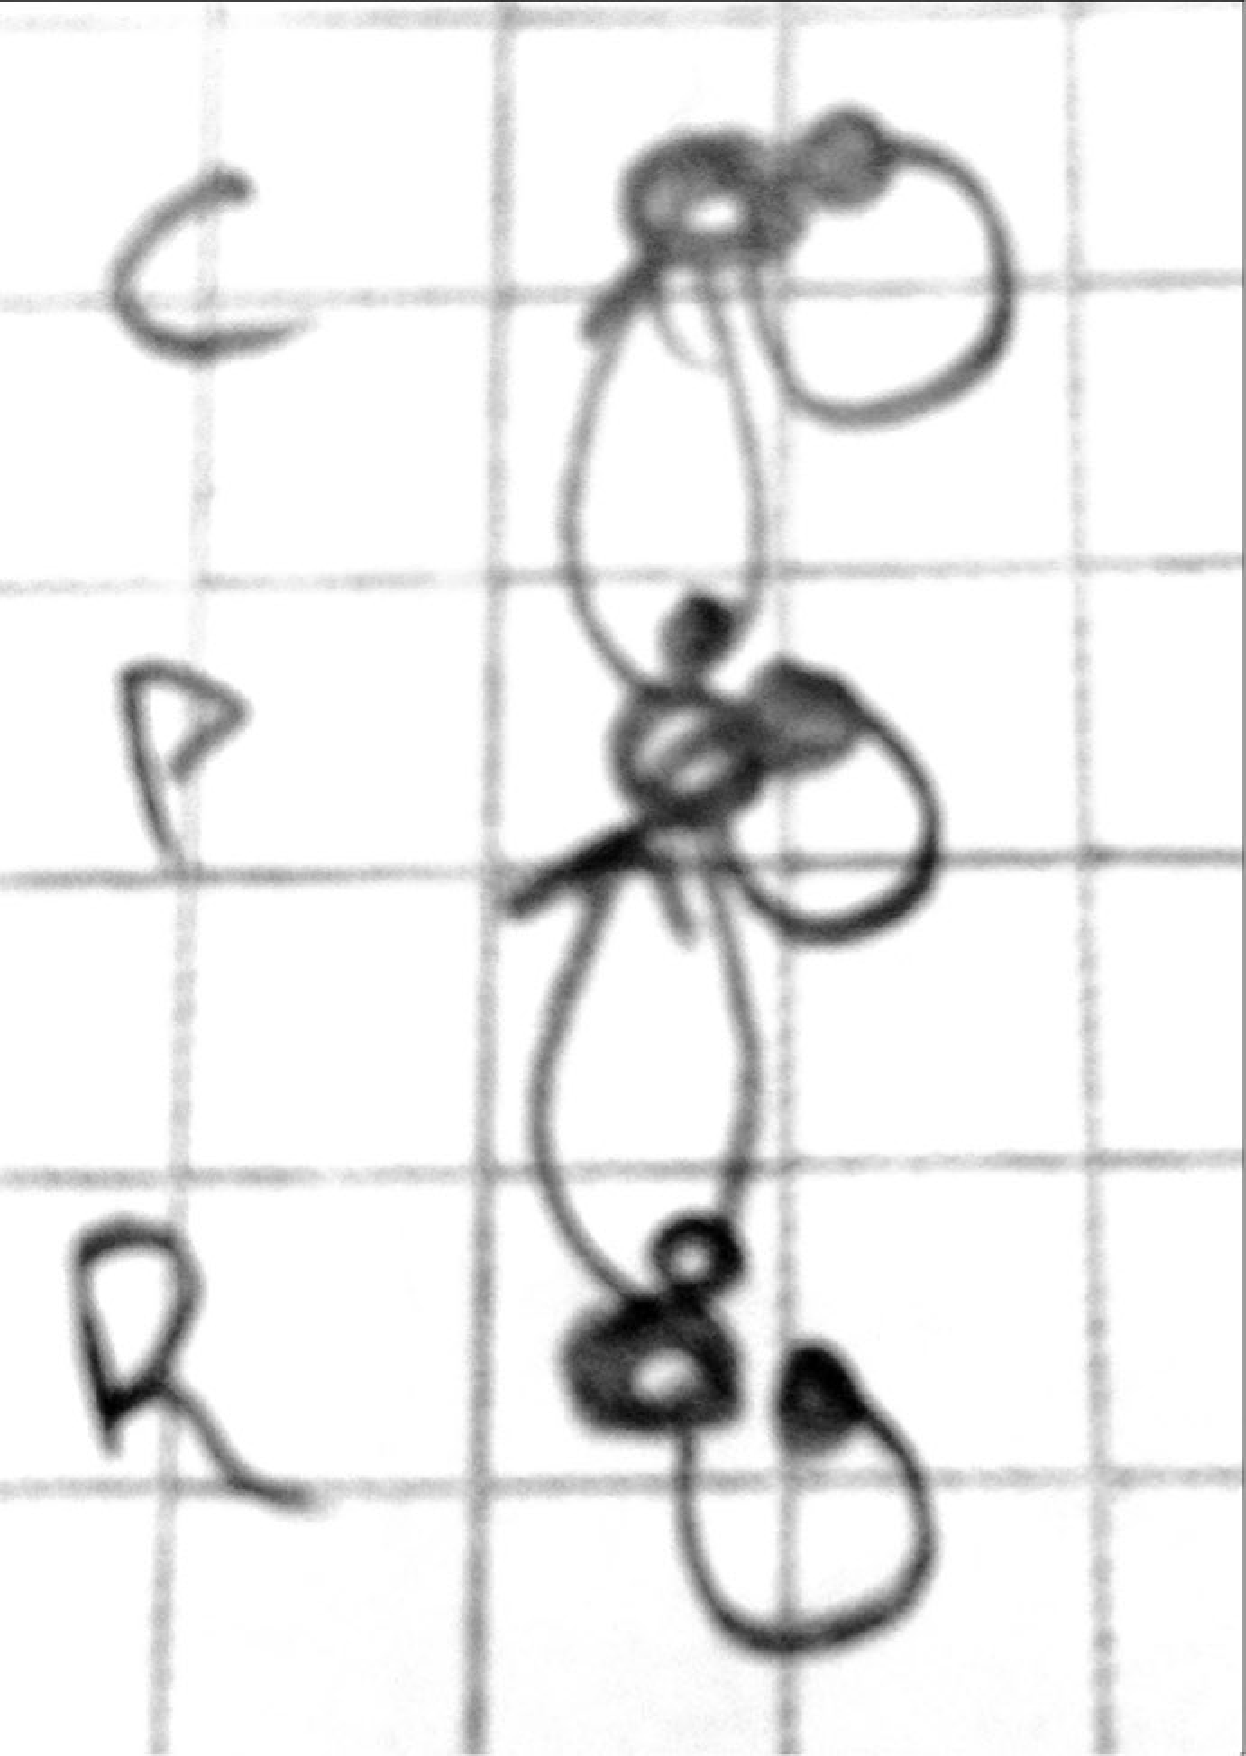
\includegraphics[width=1cm]{figs/TC_full.pdf}
\note{$\Rightarrow$ Mathematica}
\begin{align*}
	\mathbf{A}&=\begin{bmatrix} -A_{11} & -A_{12} & 0 \\ \phantom{-}A_{21} & -A_{22} & -A_{23} \\ 0 & \phantom{-}A_{32} & -A_{33} \end{bmatrix} \qquad \Rightarrow \qquad \\
	\mathbf{A^{-1}}&=
	\begin{bmatrix}
 \frac{A_{23} A_{32}+A_{22} A_{33}}{det(\mathbf{A})} & -\frac{A_{12} A_{33}}{det(\mathbf{A})} & \frac{A_{12} A_{23}}{det(\mathbf{A})} \\
 \frac{A_{21} A_{33}}{det(\mathbf{A})} & \frac{A_{11} A_{33}}{det(\mathbf{A})} & -\frac{A_{11} A_{23}}{det(\mathbf{A})} \\
 \frac{A_{21} A_{32}}{det(\mathbf{A})} & \frac{A_{11} A_{32}}{det(\mathbf{A})} & \frac{A_{12} A_{21}+A_{11} A_{22}}{det(\mathbf{A})}\end{bmatrix}\\
 \\
 det(\mathbf{A})&=-A_{11} A_{23} A_{32}-A_{12} A_{21} A_{33}-A_{11} A_{22} A_{33}
\end{align*}
Thus
\begin{align*}
	-\mathbf{A}^{-1}=-\frac{adj(\mathbf{A})}{det(\mathbf{A})}
\end{align*}
Things to notice:\\
\textbf{Determinant} is common to all elements of $\mathbf{A}^{-1}$ $\Rightarrow$ measure of community sensitivity\\
\textbf{Classical adjoint matrix} reflects \emph{magnitude and direction} of species-specific responses.\\
Species responses depend on both \emph{inter-} and \emph{intra-} specific direct effects.\\

e.g., How Resource responds to Intermediate Consumer depends on  $A_{12} \times A_{33}$.\\
Resource will affect Consumer only if Top Predator doesn't increase in abundance and eat more Consumers!\\
e.g., How Resource responds to positive press of itself is affected by self-limitation of both predators!


\rule[0.5ex]{\linewidth}{1pt}

\textbf{Symbolic Inverse of IGP}\\
\emph{\textbf{Self-limitation basal species}}\\
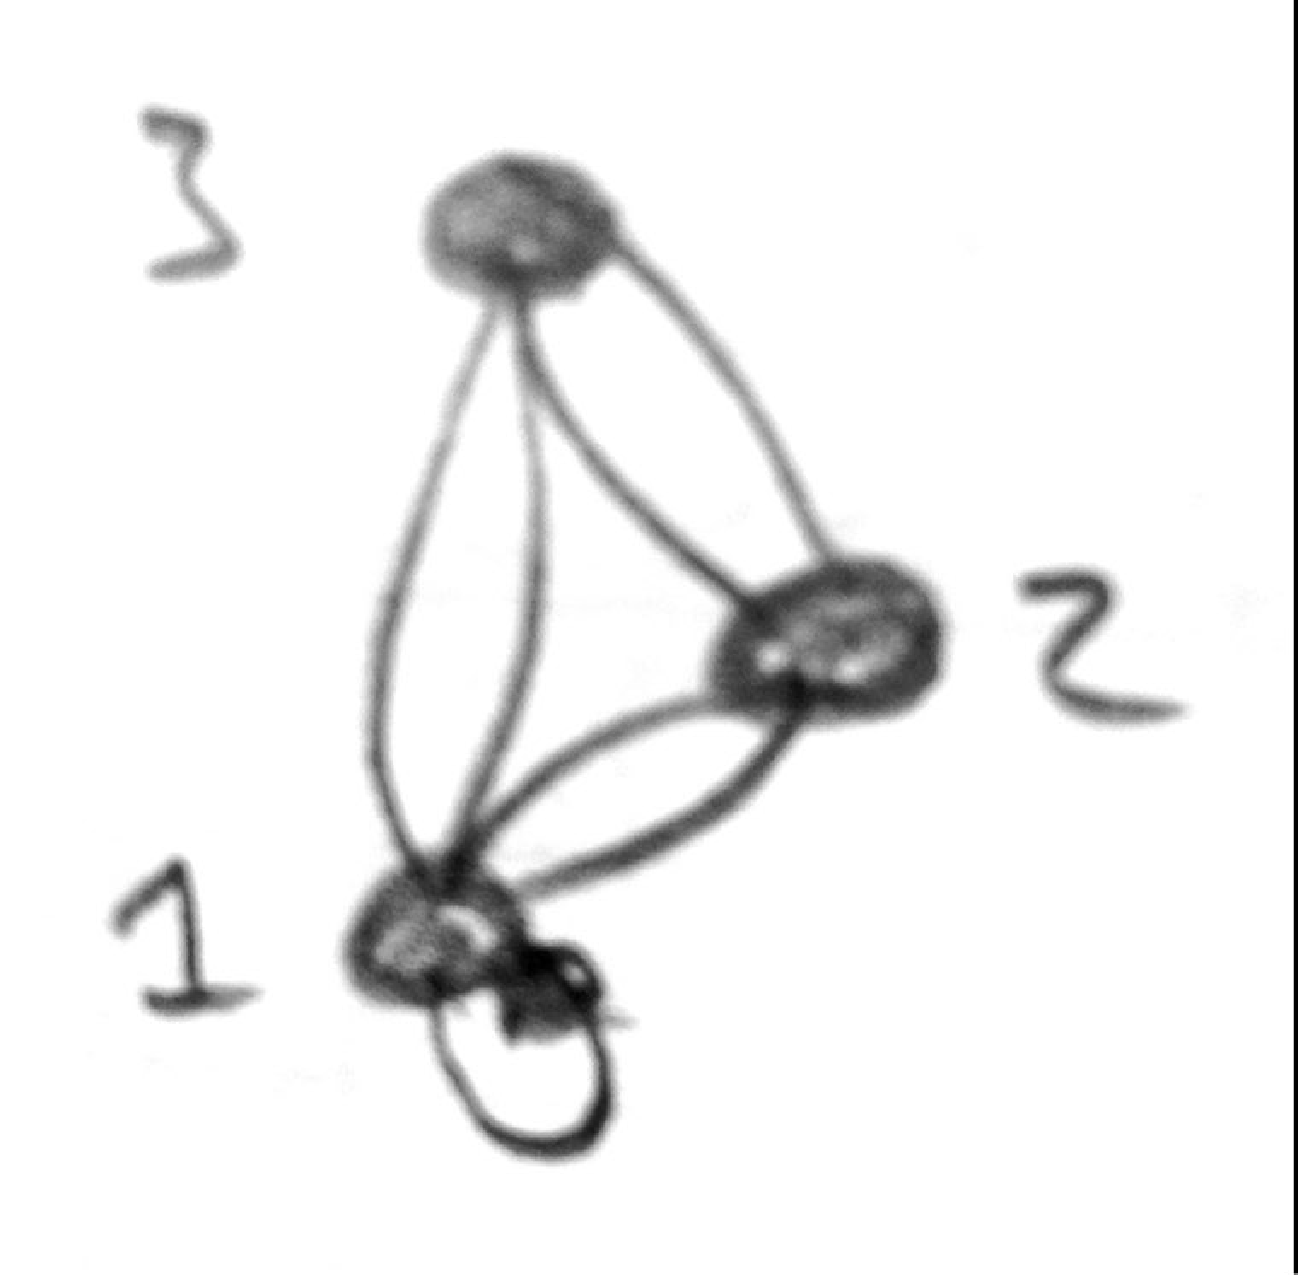
\includegraphics[width=1.25cm]{figs/IGP_basal.pdf}
 $\Rightarrow$ Mathematica
\begin{align*}
	\mathbf{A}&=\begin{bmatrix}
	 -A_{11} & -A_{12} & -A_{13} \\
	 \phantom{-}A_{21} & 0 & -A_{23} \\
	 \phantom{-}A_{31} & \phantom{-}A_{23} & 0  \end{bmatrix} \qquad \Rightarrow\\
	 adj(\mathbf{A})&=\begin{bmatrix}
	  \phantom{-}A_{23}A_{23} & -A_{13} A_{23} & A_{12} A_{23} \\
	  -A_{23} A_{31} & \phantom{-}A_{13} A_{31} & \boxed{-A_{13} A_{21}-A_{11} A_{23}} \\
	  \phantom{-}A_{21} A_{23} & \boxed{A_{11} A_{23}-A_{12} A_{31}} & A_{12} A_{21}  \end{bmatrix}
\end{align*}

Things to notice:\\
Responses of Omnivore to IConsumer, and of IConsumer to Omnivore are \textbf{qualitatively indeterminate}.\\
\ind \ind  ...depend on quantitative interaction strength values.\\
\ind \ind \ind ...in particular the strength of \emph{intraspecific self-limitation in the \textbf{Resource}!}

\rule[0.5ex]{\linewidth}{1pt}
Net effects matrix is potentially very powerful if we can estimate \emph{`interaction strengths'}.\\
Gonna skip lecture on `Interaction strengths' to talk about 'Tipping points \& Early-warning signals',\\
\ind but do want to clear up confusion that's pervasive in the literature regarding three common terms:
\begin{align*}
	\text{`The Jacobian'} \quad &\Leftrightarrow \quad \text{`The Community Matrix'}\\
	\text{`The Community Matrix'}\quad &\Leftrightarrow \quad \text{`The Interaction Matrix'}
\end{align*}
Using LV-pred prey model as example

\begin{minipage}[t]{0.5\textwidth}
\begin{center}\textbf{Population growth rates}\end{center}
\begin{align*}
	\frac{dR}{dt}&=F_R = R(b-aC)\\
	\frac{dC}{dt}&=F_C=C(eaR-d)
\end{align*}
\begin{equation*}\mathbf{A}_{ij}=\frac{\partial F_i}{\partial N_j}\end{equation*}
\begin{center}\textbf{Community matrix}\\(is a Jacobian)\end{center}
\begin{align*}
	=&\begin{bmatrix}
	b-aC^* & -aR^*\\eaC^* & eaR^* - d
	\end{bmatrix}\\
	=&\begin{bmatrix}
		0 & -\frac{d}{e}\\eb & 0
		\end{bmatrix}
\end{align*}
Use this for stability analysis.\\
Remember: $F_R(R^*,C^*)=F_C(R^*,C^*)=0$\\
...making rest of analysis possible.\\
\\
$-\mathbf{A}^{-1} \Rightarrow$ perturbation of popn growth rates.
\end{minipage}
\begin{minipage}[t]{0.5\textwidth}
\begin{center}\textbf{Per capita growth rates}\end{center}
\begin{align*}
	\frac{1}{R}\frac{dR}{dt}&=f_R = b-aC\\
	\frac{1}{C}\frac{dC}{dt}&=f_C=eaR-d
\end{align*}
\begin{equation*}\mathbf{A}_{ij}=\frac{\partial f_i}{\partial N_j}\end{equation*}
\begin{center}\textbf{Interaction matrix}\\(is a Jacobian)\end{center}
\begin{align*}
\\
\\
	=&\begin{bmatrix}
		0 & -a\\ea & 0
		\end{bmatrix}
\end{align*}
Doesn't have same stability properties.\\
But, if `D-Stable'$\Rightarrow$ Community matrix also stable.\\
\\
$-\mathbf{A}^{-1} \Rightarrow$  perturb of per capita growth rates.
\end{minipage}

\rule[0.5ex]{\linewidth}{1pt}

Press perturbation of \emph{per capita} growth rate starts with:\\
\begin{equation*}
	\frac{1}{N_1}\frac{dN_1}{dt}=f_1(\vec{N}^*)+p_1 \qquad \qquad  \frac{1}{N_2}\frac{dN_2}{dt}=f_2(\vec{N}^*)
\end{equation*}

\rule[0.5ex]{\linewidth}{1pt}

Press perturbation of population sizes:\\
\ind $\Rightarrow$ \emph{Normalized Net Effects matrix}
\begin{align*}
\hat{\mathbf{A}}^{-1}=\frac{A_{ij}^{(-1)}}{A_{ii}^{(-1})}=\frac{\frac{\partial N_i^*}{\partial p_j}}{\frac{\partial N_j^*}{\partial p_j}}=\frac{\partial N_i^*}{\partial N_j^*}
\end{align*}



\rule[0.5ex]{\linewidth}{1pt}

\end{document}